\documentclass[tikz,border=1mm]{standalone}
\usepackage[utf8]{inputenc}
\usetikzlibrary{arrows,shadows,positioning,shapes.geometric}

% colors
\definecolor{myblue}{rgb}{0.4, 0.6, 0.8}
\definecolor{mycoral}{rgb}{0.97,0.51,0.47}
\definecolor{mygreen}{rgb}{0.66,0.89,0.63}
\definecolor{myocra}{rgb}{1, 0.8, 0.4}
\definecolor{mypurple}{rgb}{0.7, 0.6, 0.9}

\tikzset{
  frame/.style={rectangle, draw, text width=6.0cm, text centered, minimum height=1.2cm, drop shadow, rounded corners},
  arrow/.style={draw, -latex, rounded corners=3mm, line width=1mm},
  line/.style={draw, line width=1cm},
  tag/.style={rectangle, draw, text width=0.75cm, text centered, minimum height=0.2cm}
}

\begin{document}

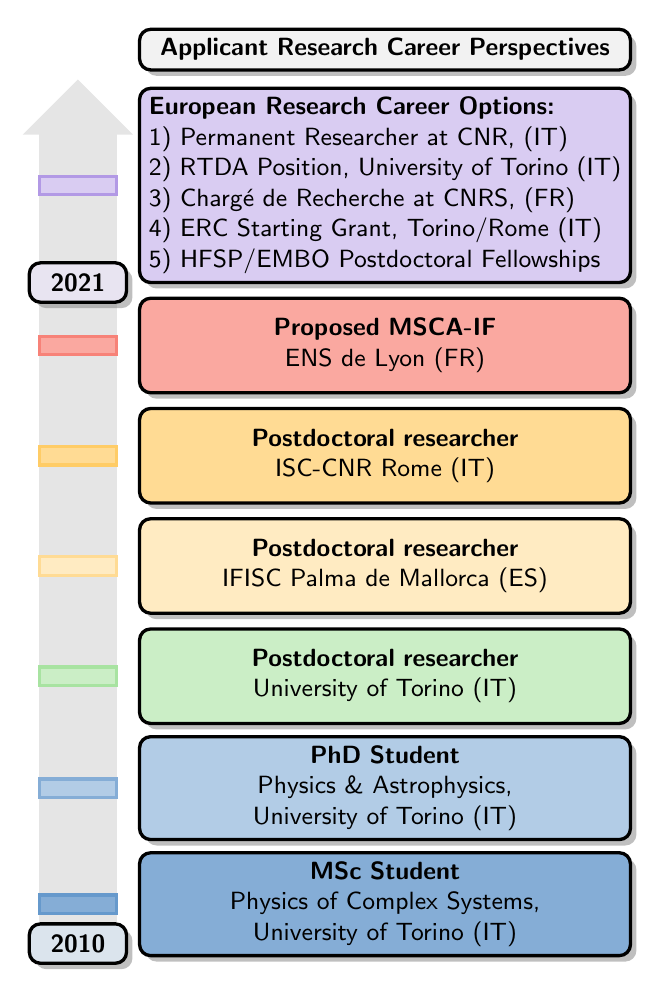
\begin{tikzpicture}[font=\small\sffamily,very thick,node distance = 3.9cm]

\draw[ -triangle 90, gray!20, line width=2.2mm, postaction={draw, line width=1.0cm, shorten >=0.5cm, -}] 
(-3.9,-1.7) -- (-3.9,9.0);

%\draw[ -triangle 90, gray!40, line width=1.5mm, postaction={draw, line width=0.4cm, shorten >=0.2cm, -}] 
%(-3.9,6.5) -- (-3.9,9.0);

% boxes
\node [frame, fill=myblue!80, below=0.8cm] (master) 
{{\bfseries MSc Student}\\ Physics of Complex Systems,\\ University of Torino (IT)};
\node [tag, fill=myblue!80, draw=myblue, left of=master] (tag1) {};

\node [frame, fill=myblue!50] (phd) 
{{\bfseries PhD Student}\\ Physics \& Astrophysics, University of Torino (IT)};
\node [tag, fill=myblue!50, draw=myblue!80, left of=phd] (tag2) {};

\node [frame, above=0.8cm,  fill=mygreen!60] (postdoc1) 
{{\bfseries Postdoctoral researcher}\\ University of Torino (IT)};
\node [tag, fill=mygreen!60, draw=mygreen, left of=postdoc1] (tag3) {};

\node [frame, above=2.2cm, fill=myocra!40] (postdoc2) 
{{\bfseries Postdoctoral researcher}\\ IFISC Palma de Mallorca (ES)};
\node [tag, fill=myocra!40, draw=myocra!70, left of=postdoc2] (tag4) {};

\node [frame, above=3.6cm, fill=myocra!70] (postdoc3) 
{{\bfseries Postdoctoral researcher}\\ ISC-CNR Rome (IT)};
\node [tag, fill=myocra!70, draw=myocra, left of=postdoc3] (tag5) {};

\node [frame, above=5.0cm, fill=mycoral!70] (msca) 
{{\bfseries Proposed MSCA-IF}\\ ENS de Lyon (FR)};
\node [tag, fill=mycoral!70, draw=mycoral, left of=msca] (tag6) {};

\node [frame, above=6.4cm, fill=mypurple!50, text justified] (options) {
{\bfseries European Research Career Options:}\\
1) Permanent Researcher at CNR, (IT)\\
2) RTDA Position, University of Torino (IT)\\
3) Charg\'e de Recherche at CNRS, (FR)\\
4) ERC Starting Grant, Torino/Rome (IT)\\
5) HFSP/EMBO Postdoctoral Fellowships
};
\node [tag, fill=mypurple!50, draw=mypurple, left of=options] (tag7) {};

% data
\node [frame, below=0.5cm, text width=1cm, minimum height=0.5cm, fill=gray!30!myblue!25, left of=master] 
(2010) {{\bfseries 2010}};

\node [frame, above=0.8cm, text width=1cm, minimum height=0.5cm, fill=gray!30!mypurple!25, left of=msca] 
(2021) {{\bfseries 2021}};

\node [frame, above=9.1cm, text width=6cm, minimum height=0.5cm, fill=gray!10, ] (date) 
{{\bfseries Applicant Research Career Perspectives}};

\end{tikzpicture}

\end{document}